\documentclass[noauthor,nooutcomes,handout,hints,12pt]{ximera}
\graphicspath{  
{./}
{./whoAreYou/}
{./drawingWithTheTurtle/}
{./bisectionMethod/}
{./circles/}
{./anglesAndRightTriangles/}
{./lawOfSines/}
{./lawOfCosines/}
{./plotter/}
{./staircases/}
{./pitch/}
{./qualityControl/}
{./symmetry/}
{./nGonBlock/}
}


%% page layout
\usepackage[cm,headings]{fullpage}
\raggedright
\setlength\headheight{13.6pt}


%% fonts
\usepackage{euler}

\usepackage{FiraMono}
\renewcommand\familydefault{\ttdefault} 
\usepackage[defaultmathsizes]{mathastext}
\usepackage[htt]{hyphenat}

\usepackage[T1]{fontenc}
\usepackage[scaled=1]{FiraSans}

%\usepackage{wedn}
\usepackage{pbsi} %% Answer font


\usepackage{cancel} %% strike through in pitch/pitch.tex


%% \usepackage{ulem} %% 
%% \renewcommand{\ULthickness}{2pt}% changes underline thickness

\tikzset{>=stealth}

\usepackage{adjustbox}

\setcounter{titlenumber}{-1}

%% journal style
\makeatletter
\newcommand\journalstyle{%
  \def\activitystyle{activity-chapter}
  \def\maketitle{%
    \addtocounter{titlenumber}{1}%
                {\flushleft\small\sffamily\bfseries\@pretitle\par\vspace{-1.5em}}%
                {\flushleft\LARGE\sffamily\bfseries\thetitlenumber\hspace{1em}\@title \par }%
                {\vskip .6em\noindent\textit\theabstract\setcounter{question}{0}\setcounter{sectiontitlenumber}{0}}%
                    \par\vspace{2em}
                    \phantomsection\addcontentsline{toc}{section}{\thetitlenumber\hspace{1em}\textbf{\@title}}%
                     }}
\makeatother



%% thm like environments
\let\question\relax
\let\endquestion\relax

\newtheoremstyle{QuestionStyle}{\topsep}{\topsep}%%% space between body and thm
		{}                      %%% Thm body font
		{}                              %%% Indent amount (empty = no indent)
		{\bfseries}            %%% Thm head font
		{)}                              %%% Punctuation after thm head
		{ }                           %%% Space after thm head
		{\thmnumber{#2}\thmnote{ \bfseries(#3)}}%%% Thm head spec
\theoremstyle{QuestionStyle}
\newtheorem{question}{}



\let\freeResponse\relax
\let\endfreeResponse\relax

%% \newtheoremstyle{ResponseStyle}{\topsep}{\topsep}%%% space between body and thm
%% 		{\wedn\bfseries}                      %%% Thm body font
%% 		{}                              %%% Indent amount (empty = no indent)
%% 		{\wedn\bfseries}            %%% Thm head font
%% 		{}                              %%% Punctuation after thm head
%% 		{3ex}                           %%% Space after thm head
%% 		{\underline{\underline{\thmname{#1}}}}%%% Thm head spec
%% \theoremstyle{ResponseStyle}

\usepackage[tikz]{mdframed}
\mdfdefinestyle{ResponseStyle}{leftmargin=1cm,linecolor=black,roundcorner=5pt,
, font=\bsifamily,}%font=\wedn\bfseries\upshape,}


\ifhandout
\NewEnviron{freeResponse}{}
\else
%\newtheorem{freeResponse}{Response:}
\newenvironment{freeResponse}{\begin{mdframed}[style=ResponseStyle]}{\end{mdframed}}
\fi



%% attempting to automate outcomes.

%% \newwrite\outcomefile
%%   \immediate\openout\outcomefile=\jobname.oc
%% \renewcommand{\outcome}[1]{\edef\theoutcomes{\theoutcomes #1~}%
%% \immediate\write\outcomefile{\unexpanded{\outcome}{#1}}}

%% \newcommand{\outcomelist}{\begin{itemize}\theoutcomes\end{itemize}}

%% \NewEnviron{listOutcomes}{\small\sffamily
%% After answering the following questions, students should be able to:
%% \begin{itemize}
%% \BODY
%% \end{itemize}
%% }
\usepackage[tikz]{mdframed}
\mdfdefinestyle{OutcomeStyle}{leftmargin=2cm,rightmargin=2cm,linecolor=black,roundcorner=5pt,
, font=\small\sffamily,}%font=\wedn\bfseries\upshape,}
\newenvironment{listOutcomes}{\begin{mdframed}[style=OutcomeStyle]After answering the following questions, students should be able to:\begin{itemize}}{\end{itemize}\end{mdframed}}



%% my commands

\newcommand{\snap}{{\bfseries\itshape\textsf{Snap!}}}
\newcommand{\flavor}{\link[\snap]{https://snap.berkeley.edu/}}
\newcommand{\mooculus}{\textsf{\textbf{MOOC}\textnormal{\textsf{ULUS}}}}


\usepackage{tkz-euclide}
\tikzstyle geometryDiagrams=[rounded corners=.5pt,ultra thick,color=black]
\colorlet{penColor}{black} % Color of a curve in a plot



\ifhandout\newcommand{\mynewpage}{\newpage}\else\newcommand{\mynewpage}{}\fi


\title{Einstein tilings}
\author{Bart Snapp}

\begin{document}
\begin{abstract}
We learn of recently discovered mathematics.
\end{abstract}
\maketitle

\begin{listOutcomes}
\item Think about map-coloring problems.
\item Understand why it is called an ``einstein'' tiling.
\item Think about aperiodic tilings.
\item Tell others about aperiodic tilings.
\end{listOutcomes}
Images for this activity were taken from this page:
\begin{center}
  \url{https://divisbyzero.com/2023/06/04/3d-printable-aperiodic-monotiles-and-aperiodic-monotile-coloring-book-pages/}
\end{center}
and were created by David Richeson (divisbyzero.com).


\mynewpage


\begin{question}
  New math is being created all the time. Here are two DIFFICULT math
  problems that were ``recently'' solved:
  \begin{description}
  \item[Four Color Problem] Imagine you have a map of a country or a
    region, and you want to color it in a way that no two neighboring
    areas (like states or counties) have the same color. This means
    that if two areas share a border, they must be colored
    differently. How few colors does it take?
  \item[Einstein Tiling Problem] Is it possible to take these shapes
    and tile them in a way that covers a flat surface, but no matter
    how you try, you can't create a repeating pattern that goes on
    forever without any gaps or overlaps?
  \end{description}
  When were they solved? Why is it called the ``four color'' problem? Why is it called the ``einstein tiling'' problem?
\end{question}

  
\mynewpage



\begin{question}
  Here is a tiling with the \textbf{spectre}.
  \begin{center}
    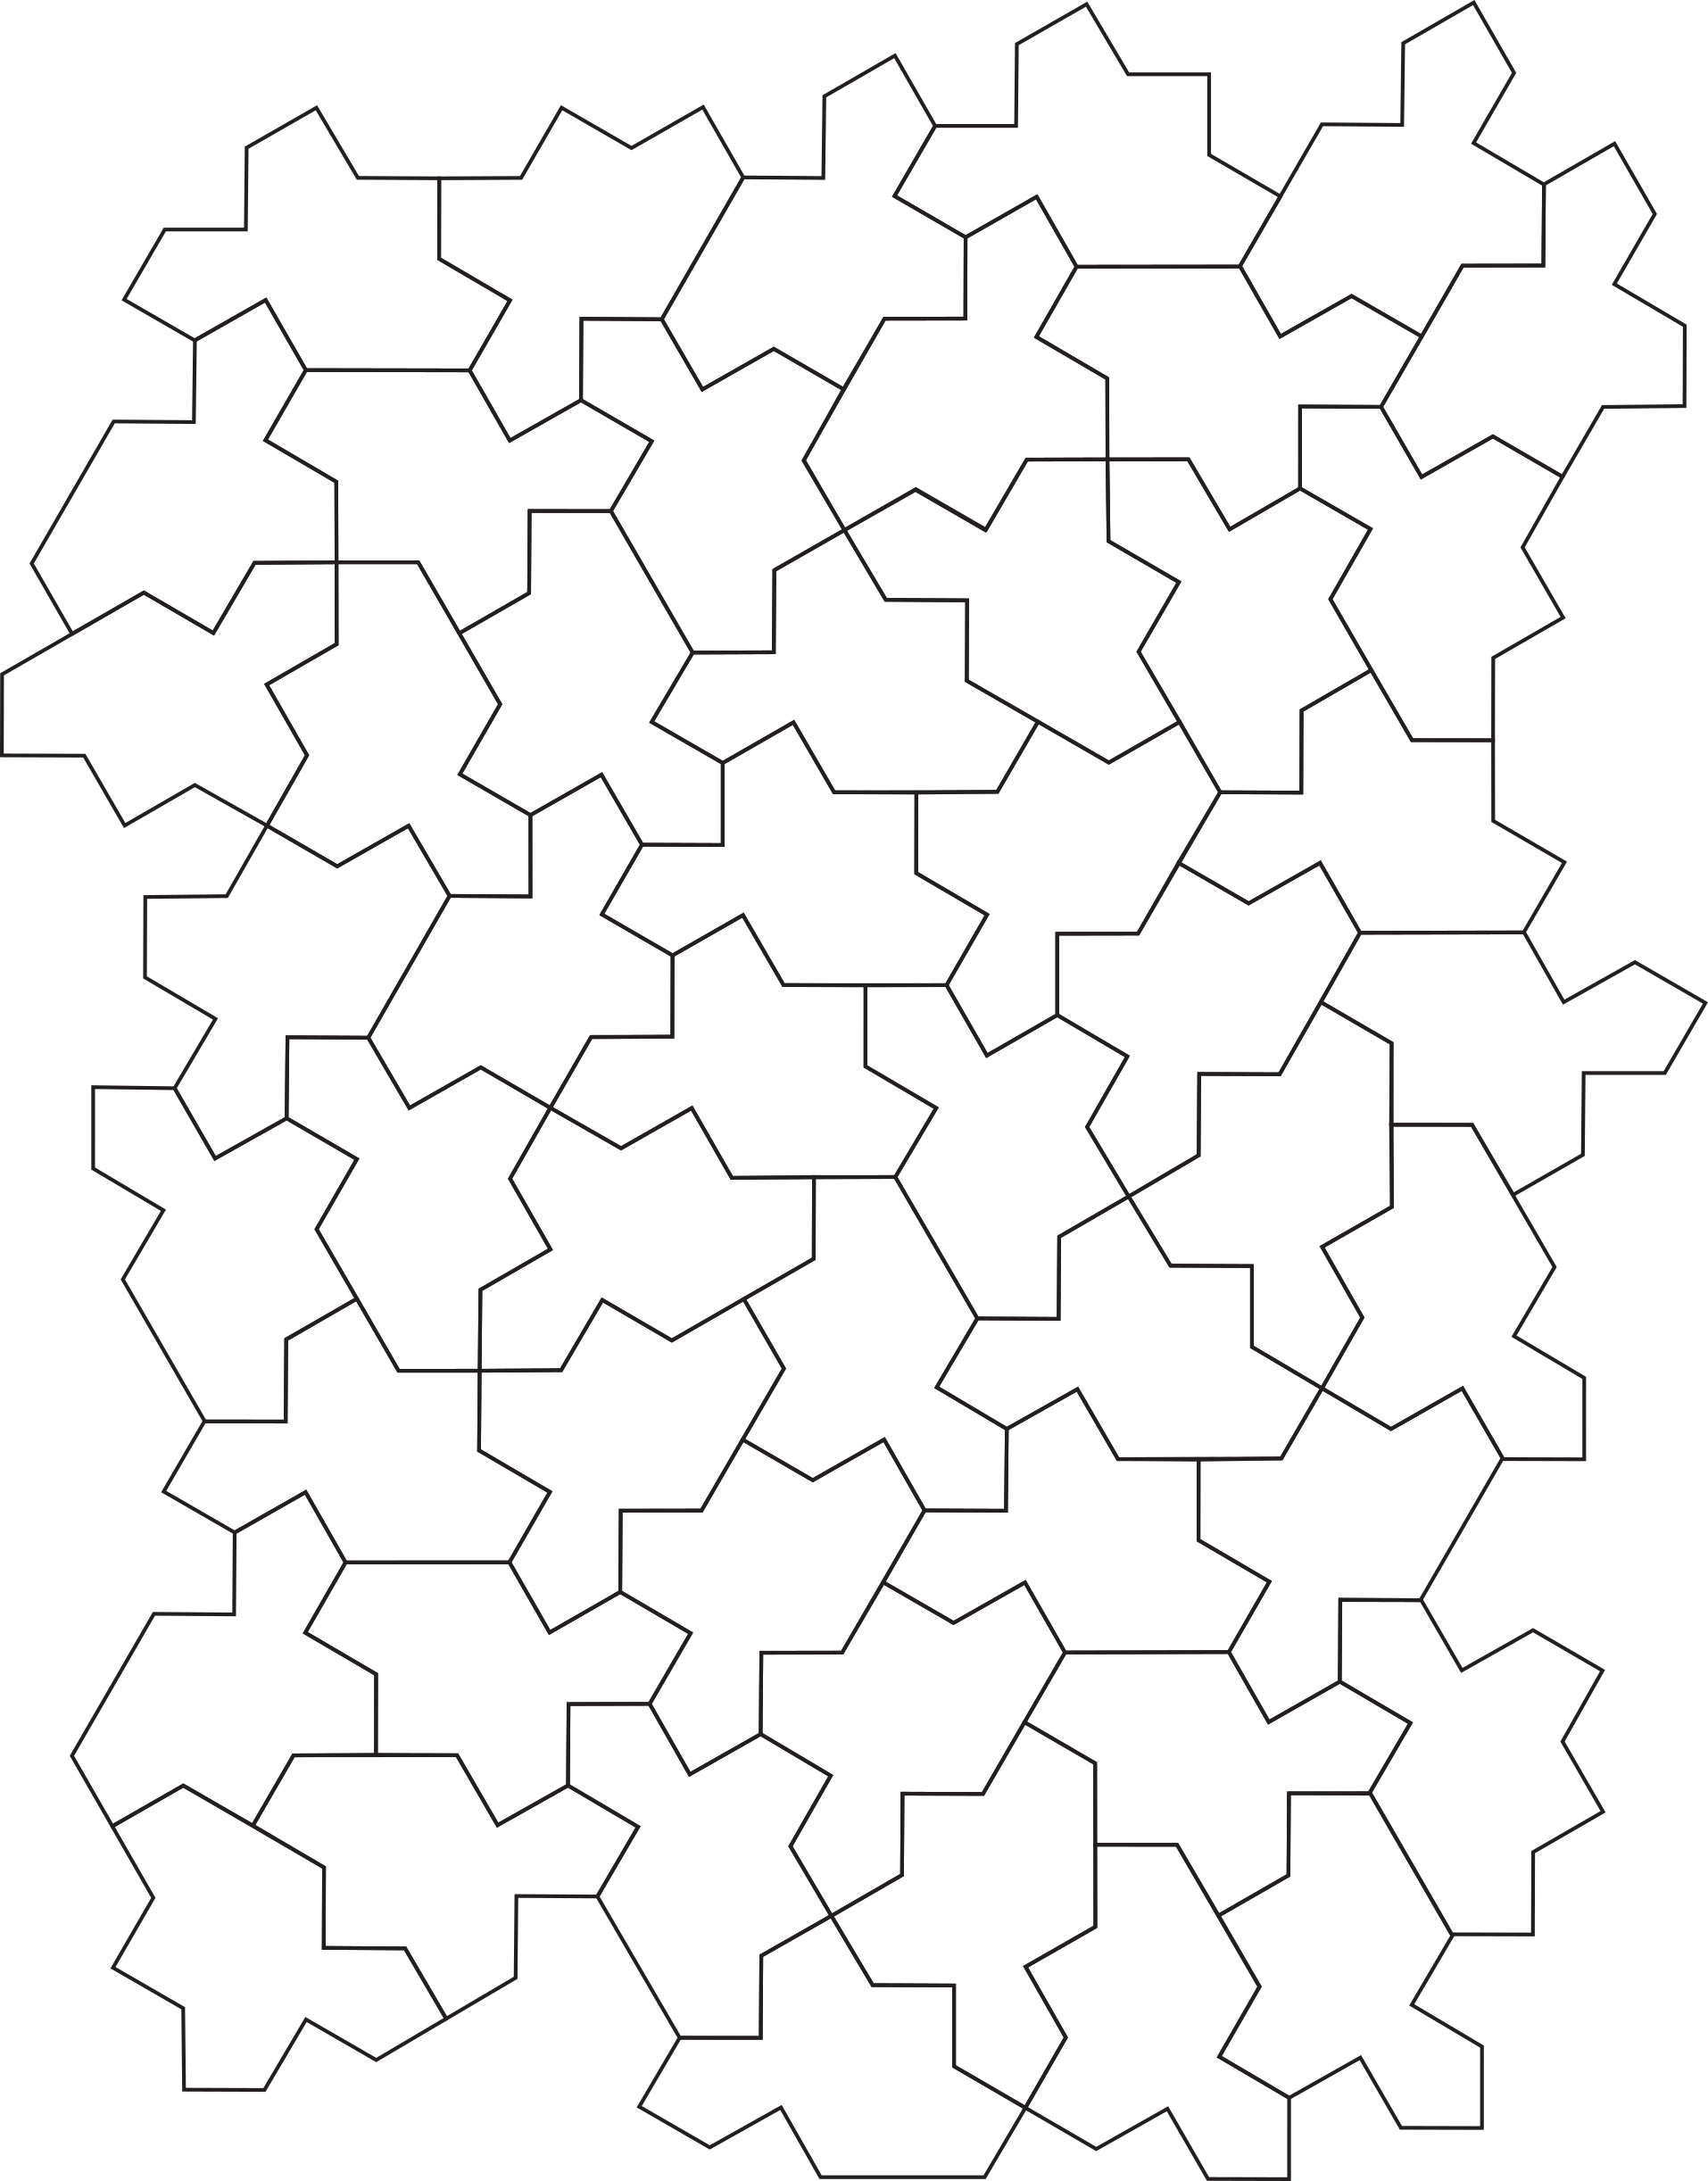
\includegraphics[scale=.9]{spectre.png}
  \end{center}
  Make this BEAUTIFUL by coloring it in with as few colors as possible
  and no adjacent tiles having the same color.
\end{question}

\mynewpage

\begin{question}
  Here is a tiling with the \textbf{hat}, and its reflection:
  \begin{center}
    left-bump hat~\raisebox{-1em}{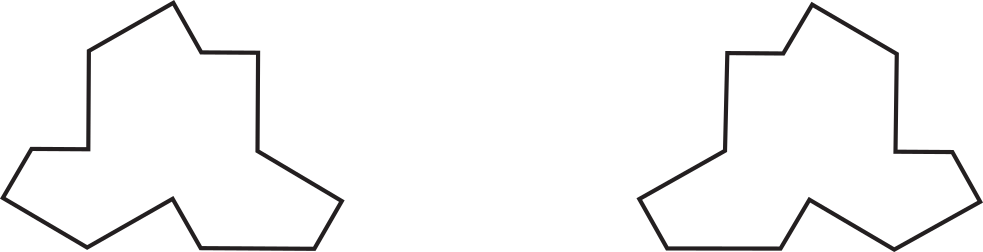
\includegraphics[scale=.8]{lrHat.png}} right-bump hat
  \end{center}
  The left-bump hat is less common than the right-bump hat on the in
  the tiling below:
  \begin{center}
    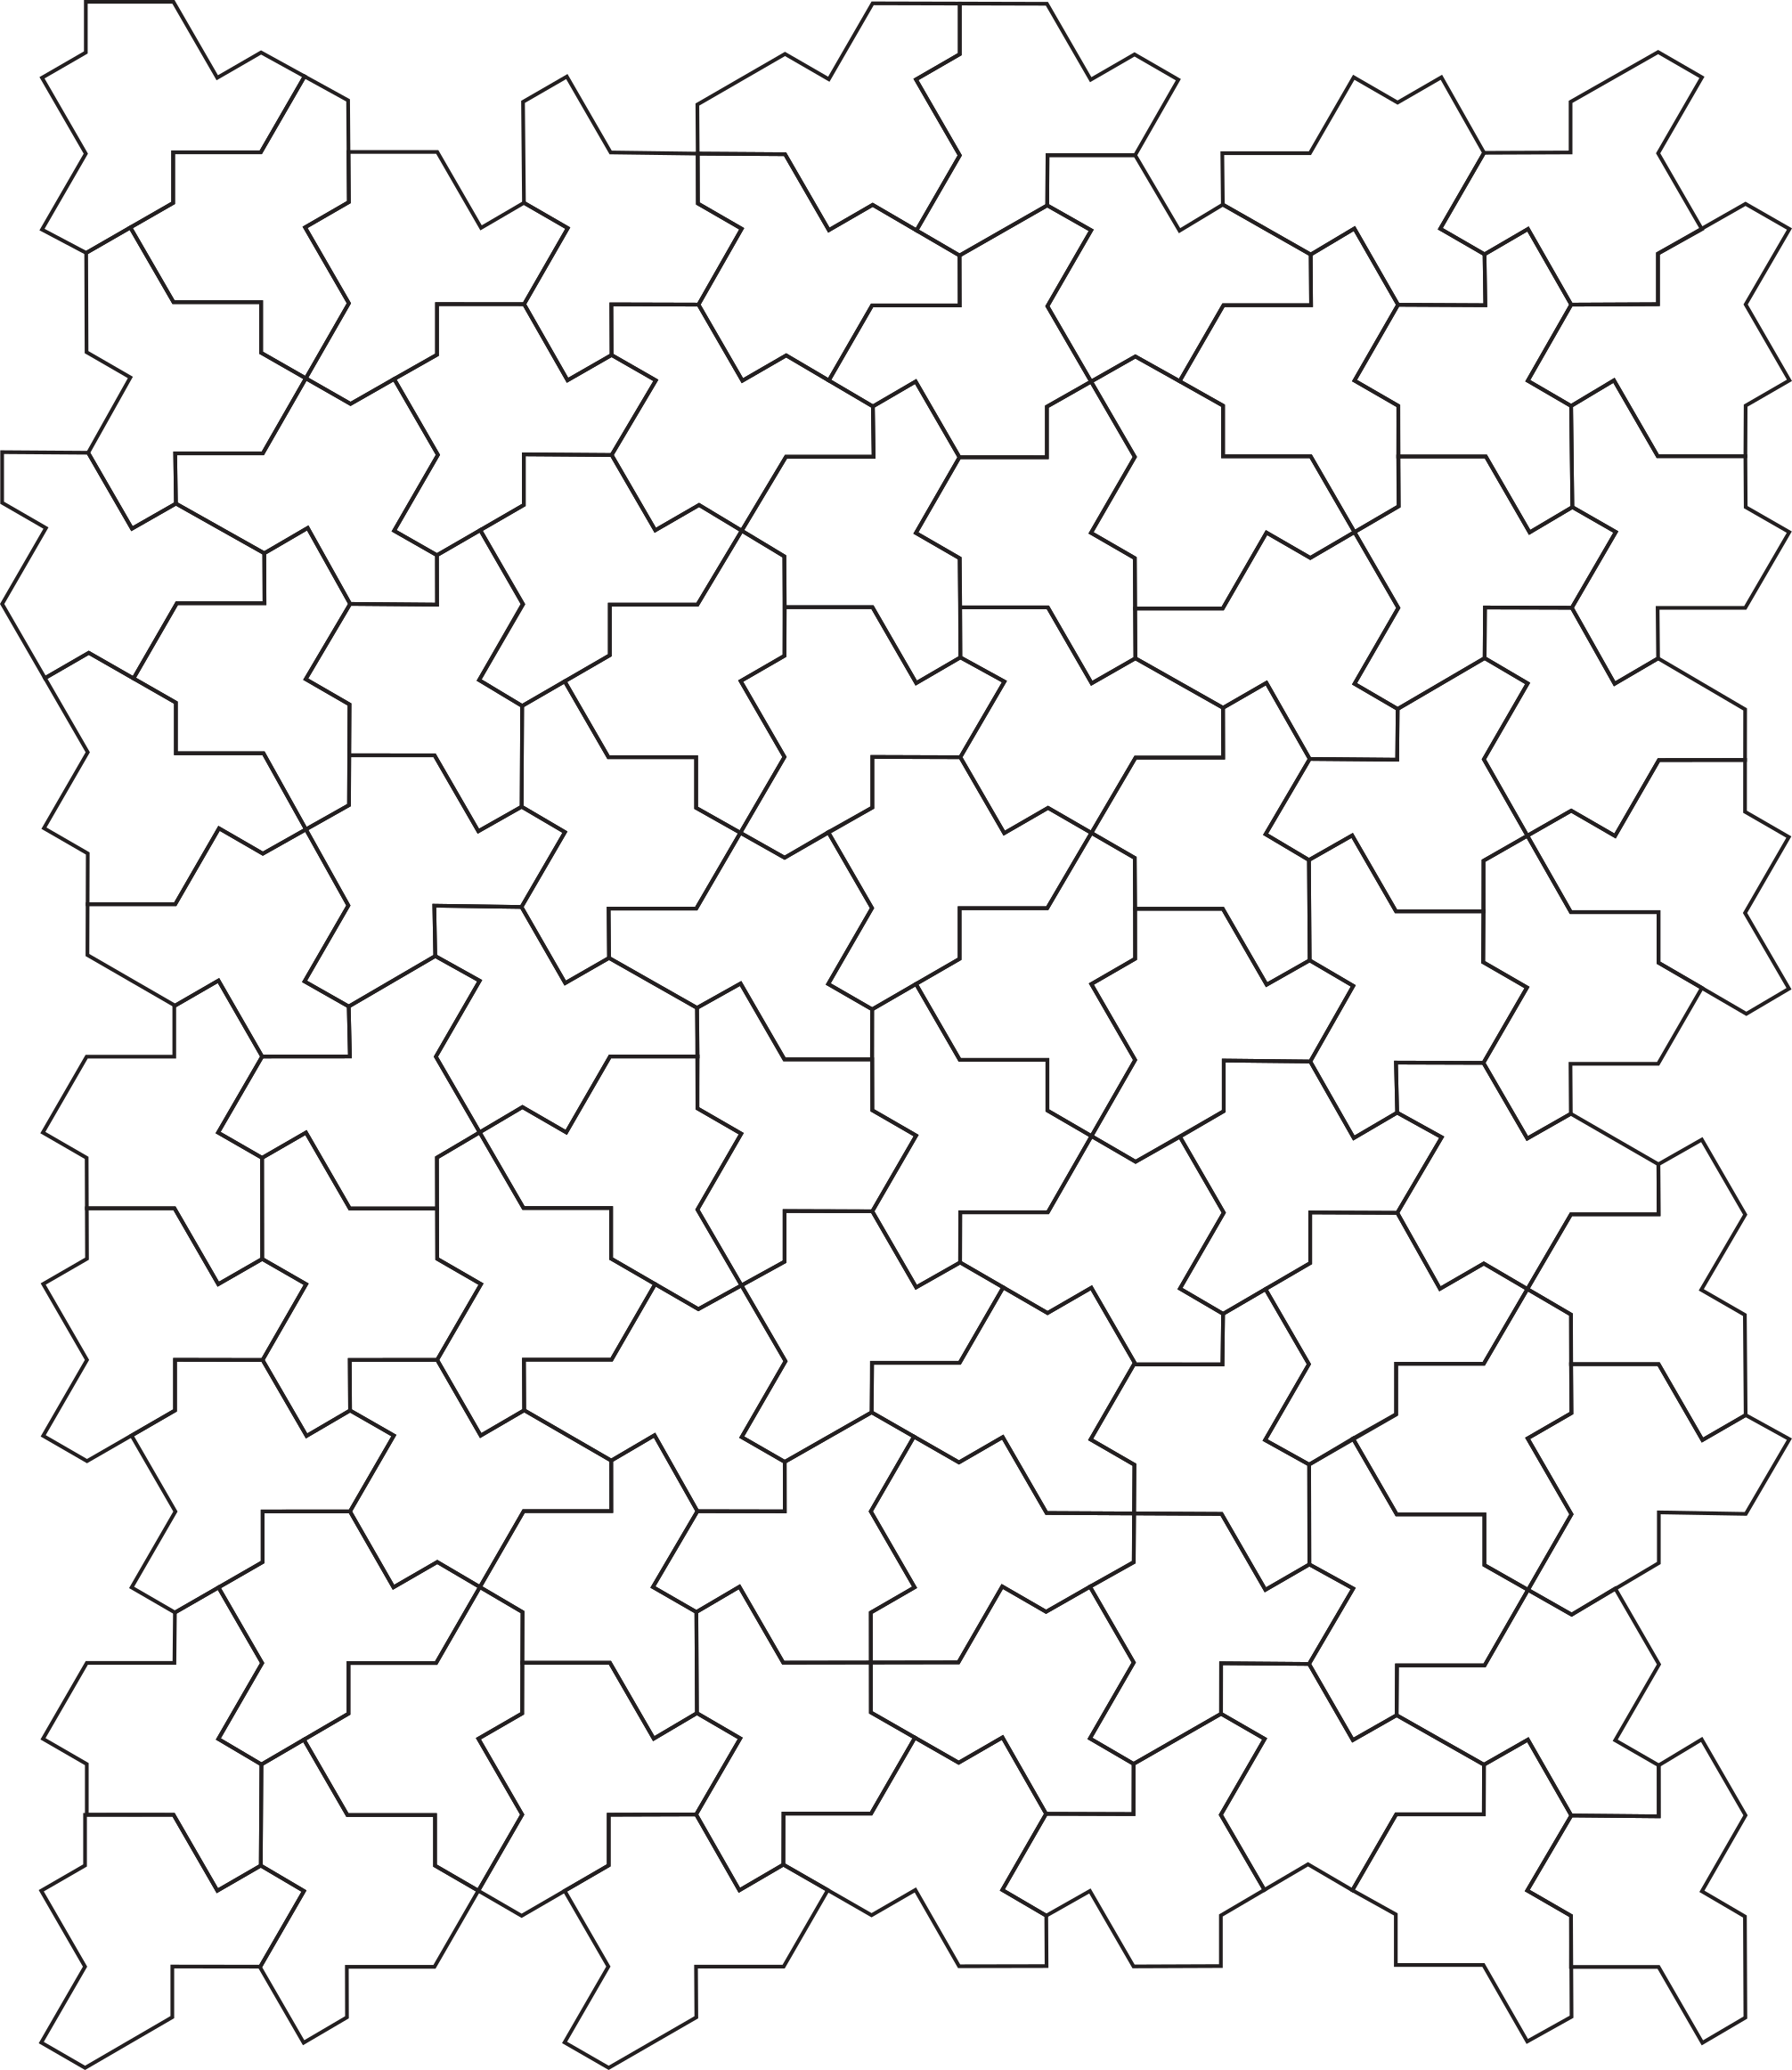
\includegraphics[scale=.8]{hat.png}
  \end{center}
  Make this BEAUTIFUL by coloring it in with as few colors as possible, no adjacent tiles having the same color, and with all of the the
  left-bump hats the SAME color. \textbf{What do you think, is the ``hat'' an einstein tile? EXPLAIN the reason for your decision.}
\end{question}


\end{document}
